\documentclass[12pt, titlepage, a4paper]{article}
\usepackage[utf8]{inputenc}
\usepackage{graphicx}
\usepackage{amsmath}

\begin{document}

  \title{Flappa Freqt}
	\author{Cecilia Lagerwall - cecla125 \\ Daniel Rönnkvist - danro716 \\
			Therese Komstadius - theko867 \\ \\ Linköpings universitet}
	\date{2014-10-10}
	\maketitle

  \renewcommand*\abstractname{Sammanfattning}
  \begin{abstract}
		“Flappa Freqt” är ett spel som har skapats som ett projekt i kursen TFYA65, ht 2014 vid Linköpings universitet med syftet att få större förståelse för ämnet ljudfysik. Denna rapport redovisar hur ljudfysiken har använts för att skapa ett spel som styrs av frekvenserna från rösten. Den förklarar vilka verktyg som använts för att spela in och analysera ljud i realtid.
	\end{abstract}

  \section{Inledning}
		I denna rapport redovisas projektet “Flappa Freqt” som genomfördes i kursen Ljudfysik, TFYA65, ht 2014 vid Linköpings universitet. Syftet med projektet var att skapa ett spel där spelaren kontrollerade spelet med hjälp av rösten.

  \section{Bakgrund}
		Eftersom projektet skulle avhandla ljudfysik blev det tidigt bestämt att fokus skulle ligga på att uppta och omvandla ljud. Därför baserades grundiden för spelet på ett redan existerande koncept. Konceptet som valdes var det bakom spelet “Flappy bird”, med skillnaden att olika röstfrekvenser skulle förlytta spelobjektet i vertikalled. Det beslutades även att spelet skulle utvecklas för en enhet med inbyggd mikrofon, därför valdes Javascript som programmeringsspråk för att utveckla till en webbläsare. Javascript valdes även för att det skulle vara enklare att hitta ett färdigt spelskelett.

	\section{Metod}
		\subsection{Verktyg}
			För att alla skulle kunna jobba tillsammans med samma kod och samtidigt hålla den strukturerad valdes versionshanteringssystemet Git. Detta med hjälp av GitHub underlättade arbetet.
			\\ \\
			För att uppta ljud från mikrofonen i en webbläsare användes \textit{Web Audio API}\cite{MDN} som är ett API, \textit{application programming interface}, för Javascript. Med hjälp av detta interface kunde en ström från mikrofonen skapas och ljudet kunde sparas och bearbetas i realtid.
			\\ \\
			Bilderna till spelet skapades i Paint och Adobe Photoshop och den illustrerade grafen skapades med hjälp av Adobe Illustrator.

		\subsection{Tillvägagångssätt}
			För att inte behöva bearbeta ljudet i hela frekvensomfånget, 0 - 20 000 Hz, applicerades ett bandpassfilter på ljudströmmen. Bandpasset valdes att vara mellan 125 och 8000 Hz, detta för att den mänskliga rösten ligger mellan dessa två frekvenser\cite{freq}. Detta filter beräknades fram genom att hitta centrum mellan de två önskade gränserna. Sedan applicerades ett Q-värde vid denna punkt för att uppnå önskat frekvensband.\cite{biqf} Centrumfrekvensen beräknades fram enligt ekvation (1) med $f_1$, minsta värde och $f_2$, största värde. Q-värdet beräknades fram via ekvation (2) med centrumfrekvensen, $f_0$ och frekvensbandet, $\bigtriangleup f$.\cite{QFi}
			\\ \\
			\begin{equation}
				\cfrac{f_2 - f_1}{2} + f_1
			\end{equation}
			\\
			\begin{equation}
				Q = \cfrac{f_0}{\bigtriangleup f}
			\end{equation}
			\\
			Ljudströmmen från mikrofonen skickades genom en \textit{analyser node} vilket gav möjligheten till realtidsinformation om ljudet både i tids- och frekvensdomän. För att få ljudet i frekvensdomän använder sig noden av en fouriertransformering av ljudet och skickar ut frekvensdatan. Denna frekvensinformation kunde sedan användas för att hitta en lämplig nivå för spelet. För fouriertransformen valdes en \textit{fftsize} till 2048 för att bestämma storleken på frekvensdomänen. Men det var bara de positiva värdena som var intressanta vilket gav en halvering av denna fftsize för de givna transformerade värdena\cite{AnalyserNode}.
			\\ \\
			För att analysera ljudet sparades alla inspelade frekvenser i en buffert. Bufferten loopades sedan igenom för att hitta den frekvens med högst amplitud. Från detta amplitudvärde subtraherades ett bestämt tröskelvärde för att hitta en gränsnivå. De frekvenser som låg över denna gräns summerades och den totala summan dividerades med antalet summerade frekvenser för att få fram en medelfrekvens. (Se bild 1.) Eftersom ljudet från mikrofonen samplades med 1024 sampel/frekvensomfång över ett 20 000 Hz omfång multiplicerades medelfrekvensen med 19.5 för att få fram det riktiga frekvensvärdet.

      		\renewcommand*\figurename{Bild}
				\begin{figure}[h!]
					\centering
						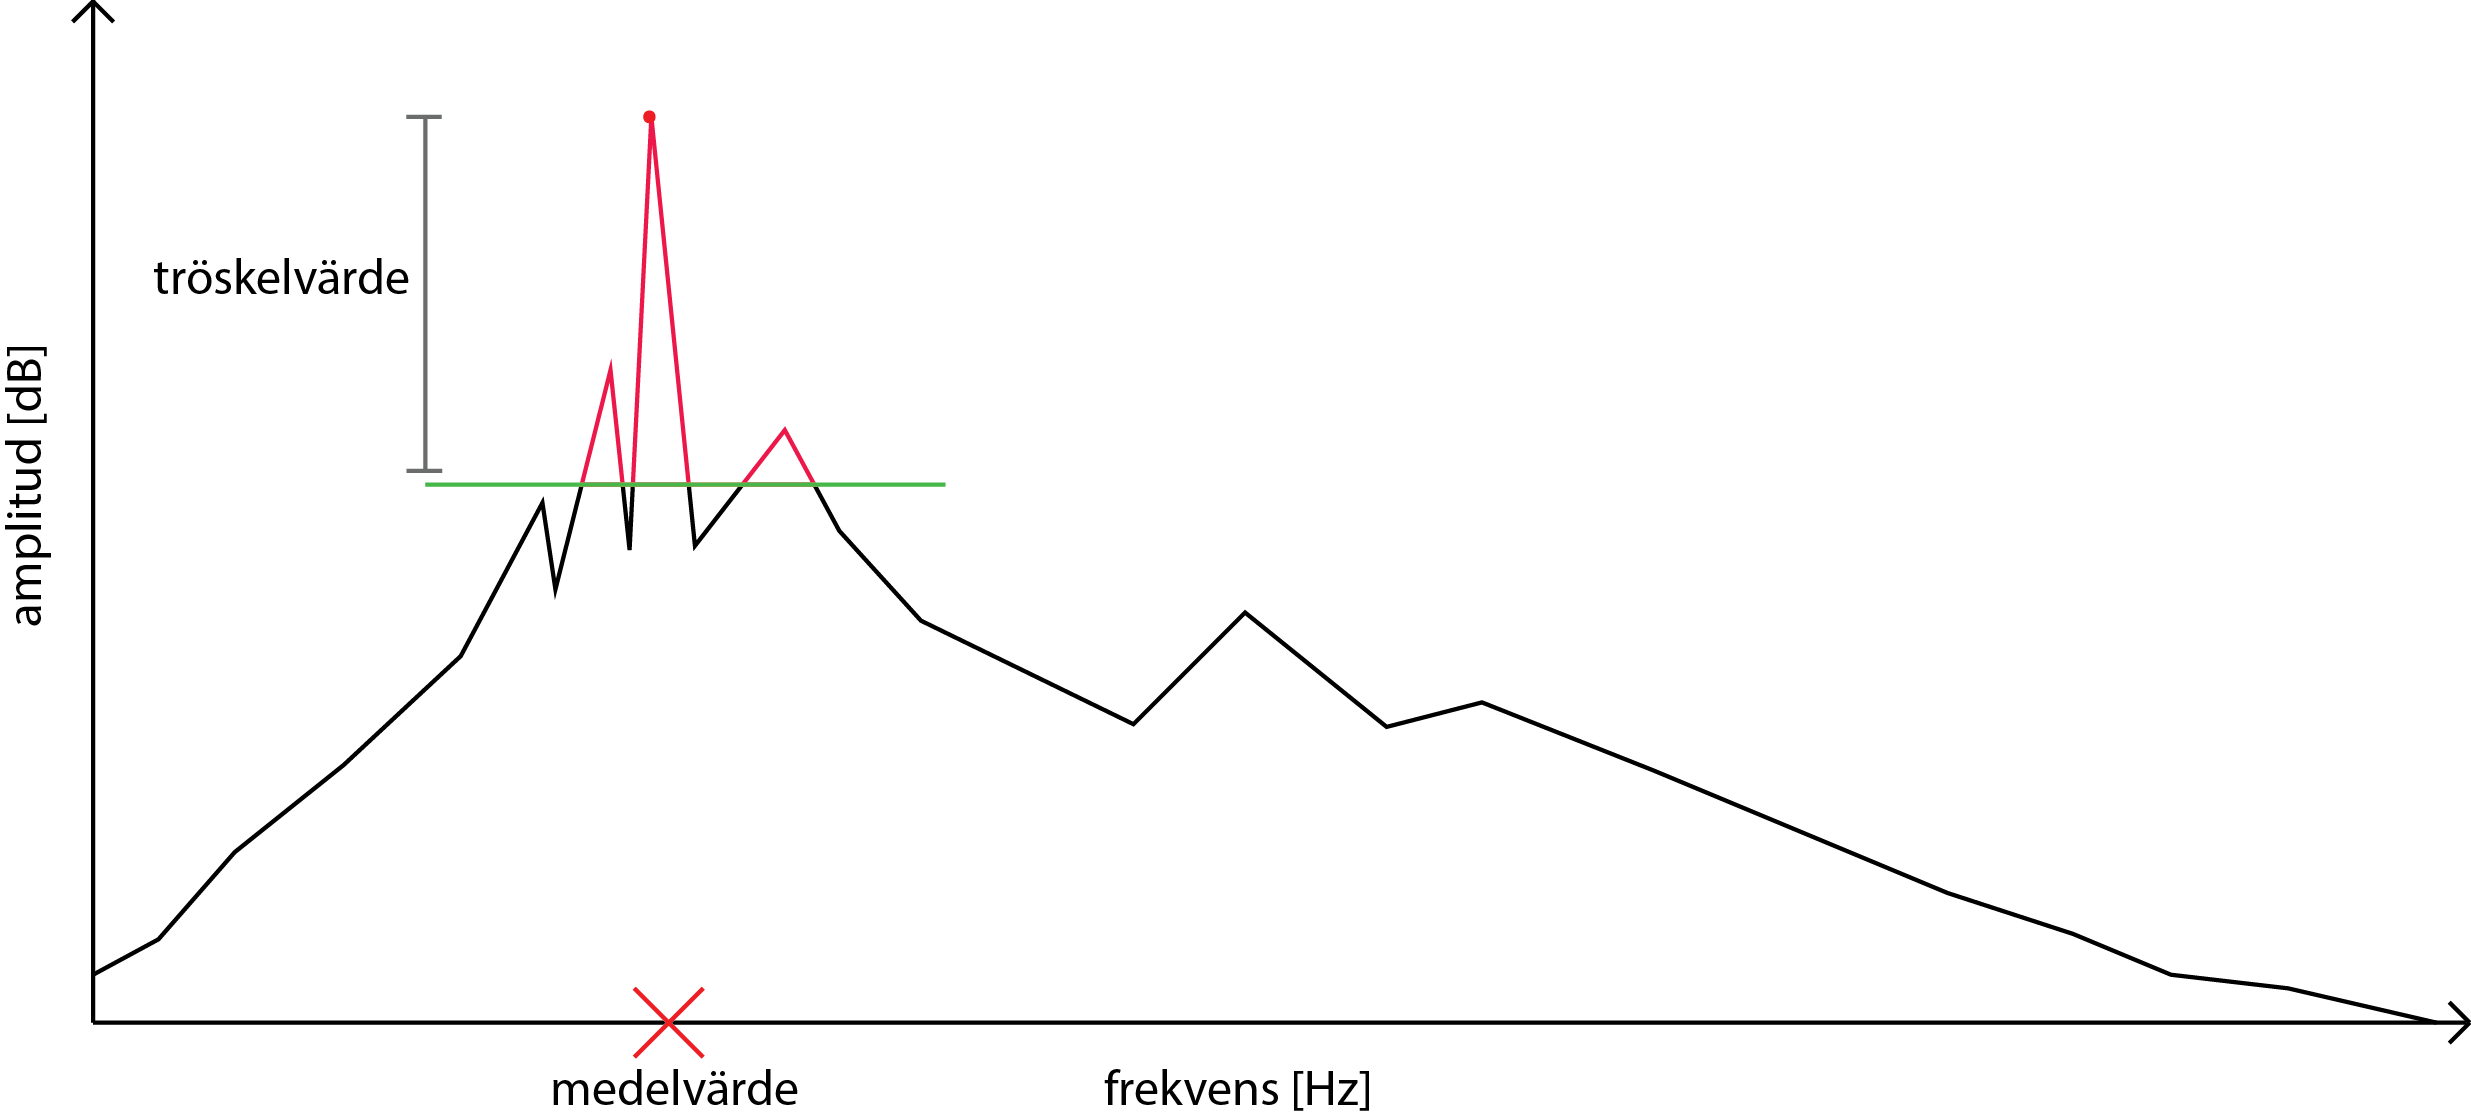
\includegraphics[width=1\textwidth]{explanation.png}
  							\caption{En illustration som förklarar hur medelfrekvensen beräknas.}
				\end{figure}
			Produkten multiplicerades därefter med en godtycklig konstant som i det här fallet valdes till två. Detta var enbart för spelupplevelsen.
			\\ \\
			Den beräknade frekvensen skickades vidare till spelet där den jämfördes med ett nollställe för att avgöra om figuren i spelet skulle åka upp eller ner. Nollstället bestämdes genom att testa olika värden och hitta ett som skapade en bra spelkontroll.

	\section{Resultat}

		Projektets resultat går att se och testa på http://tkomstadius.se/. Källkoden finns öppet på  https://github.com/danielronnkvist/flappy-wueeaaaoooo
		\\ \\
		Då spelets skelett har modifierats har en del buggar uppstått. Alla har inte åtgärdats på grund av tidsbrist.

	\section{Diskussion}
		Det fanns en del saker som hade kunnat förbättras med mer tid och bättre kunskap. Till att börja med fanns det vissa svårigheter med störningarn från bakgrundsljud. Eftersom det endast var den frekvens med högst amplitud som kontrollerade spelet kunde den frekvensen bli bestämd av anda ljud än spelarens. Detta är något som hade kunnat åtgärdas men upplevdes som svårt beroende på bakrundsljudes ljudnivå och karaktär.
		\\ \\
		För både tröskelvärdet och den lägsta tillåtna amplituden skulle det krävts fler tester för att basera dem på tidigare resultat. Det hade även varit svårt att hitta värden som skulle uppfylla alla olika typer av rum. Det hade krävt mer tid och det ansågs även vara utanför projektets ramar och lämnades därför utanför.
		\\ \\
		Hur spelet skulle styras kunde ha valts på flera olika sätt. Till exempel kunde spelet kontrollerats med ljudvolym för att bestämma om figuren skulle åka upp eller ned. Det hade även varit möjligt att använda en \textit{pitch detector} för att hitta närmaste rena ton och låta den styra. Att skapa en pitch detector var för avancerat med de kunskaper som fanns och det beslutades att det inte var nödvändigt för spelet. Fördelen med att få ut rena toner hade varit att det skulle bli enklare för spelaren. Det skulle finnas ett jämt intervall som figuren skulle förflytta sig över.
		\\ \\
		Spelet styrs helt och hållet med vilken frekvens som kommer in och inte med gravitation. Hade spelet haft en gravitation skulle det ha kunnat vara ytterligare ett moment eller svårighetsgrad i spelet. Det kunde ha räckt med att kolla om det fanns något ljud in i mikrofonen vars amplitud överskred ett visst värde. Filtrera bort brus så att bara ljud från spelaren påverkar spelet. Detta skulle ha varit en enklare variant av programmet bakom spelet. Fysiken bakom hade inte behövt vara lika nogrann och avancerad.

	\section{Slutsats}
		Målet med projektet, att kunna styra ett spel med frekvensen, uppnåddes även om spelet i sig inte fungerade helt felfritt. Mer kunskap om ljudfysik och behandling av signaler i realtid hade kunnat göra spelet mer fysikaliskt korrekt. En del variabler i programmet till spelet valdes på måfå utan någon egentlig grund. De valdes enbart för att skapa en bättre spelupplevelse. Mer tid, kunskap och tester hade kunnat göra spelet mer optimalt för dess syfte. Det fanns även en hel del buggar i spelet vilket förstörde spelupplevelsen. För att släppa spelet till en bredare publik hade dessa behövts åtgärdas först.

	\pagebreak

	\section{Referenser}
	\renewcommand{\addcontentsline}[3]{}% Remove functionality of \addcontentsline
  \renewcommand{\section}[2]{}% Remove functionality of \section
  \begin{thebibliography}{99}

  \bibitem{MDN}
    Mozilla Developer Network.
    \emph{Web Audio API.}\newline
    https://developer.mozilla.org/en-US/docs/Web/API/Web\_Audio\_API, 2014-10-07

  \bibitem{freq}
    Befria Samtalet.
    \emph{Fakta om ljudmiljö.}\newline
    http://www.befriasamtalet.se/fakta, 2014-10-08

  \bibitem{biqf}
  	Mozilla Developer Network.
    \emph{Biquad filter.}\newline
    https://developer.mozilla.org/en-US/docs/Web/API/BiquadFilterNode, 2014-10-10

  \bibitem{QFi}
    Umeås Universitet.
    \emph{Aktiva filter.}\newline
    http://www8.tfe.umu.se/courses/elektro/anakrets/TDV00/html/grupp9/, 2014-10-10

    \bibitem{AnalyserNode}
    Mozilla Developer Network.
    \emph{AnalyserNode.}\newline
    https://developer.mozilla.org/en-US/docs/Web/API/AnalyserNode, 2014-10-08

  \end{thebibliography}

\end{document}
